\documentclass[final]{beamer}
\usepackage[T1]{fontenc}
\usepackage[utf8]{inputenc}
\usepackage{lmodern}
\usepackage[size=a1,orientation=portrait,scale=1.0]{beamerposter}
\usepackage{beamerthemegemini}
\usepackage{amsmath,amssymb,booktabs,array}
\usepackage{graphicx}
\usepackage{ragged2e}
\setlength{\RaggedRightParindent}{0pt}

\title{The Informax Decoupler in ScaPre: Effects of Channel Weighting on Concept Removal and Preservation}
\author{Tse-An Li}
\institute{Department of Applied Mathematics, National Yang Ming Chiao Tung University}

\newlength{\sepwidth}
\newlength{\colwidth}
\setlength{\sepwidth}{0.025\paperwidth}
\setlength{\colwidth}{0.455\paperwidth}
\newcommand{\separatorcolumn}{\begin{column}{\sepwidth}\end{column}}
\newcommand{\tablefont}{\fontsize{22}{26}\selectfont}
\newcommand{\smalltext}{\fontsize{20}{24}\selectfont}
\newcommand{\blocktext}{\RaggedRight\setlength{\parindent}{0pt}\noindent}

\begin{document}
\begin{frame}[t]

\begin{beamercolorbox}[wd=\paperwidth,sep=1.15cm,leftskip=0.8cm,rightskip=0.8cm]{headline}
{\color{white}\bfseries\fontsize{49}{54}\selectfont
The Informax Decoupler in ScaPre:\par
Effects of Channel Weighting on Concept Removal\par
and Preservation\par}
\vspace{0.45cm}
{\color{white}\fontsize{28}{33}\selectfont
Tse-An Li \quad | \quad Advisors: Te-Sheng Lin, Jia-Wei Liao\par}
{\color{white}\fontsize{22}{27}\selectfont
Department of Applied Mathematics, National Yang Ming Chiao Tung University
\quad | \quad an.sc13@nycu.edu.tw\par}
\end{beamercolorbox}

\vspace{0.45cm}
\begin{columns}[t,totalwidth=\paperwidth]

\separatorcolumn
\begin{column}{\colwidth}

\begin{block}{1\quad Background and Question}
\blocktext
ScaPre (\textbf{Scalable and Precise Concept Unlearning}) is a closed-form method that edits cross-attention projections to remove selected concepts while preserving related content.

The \textbf{Informax Decoupler} is its channel-weighting component. It uses \textbf{mutual information (MI)}, which measures the dependence between a binarized channel activation and the target-versus-neutral label.

We ask whether these weights meaningfully distinguish channels and whether that distinction matters at image level.
\end{block}

\begin{block}{2\quad From Activations to MI Weights}
\blocktext
We follow activations $\rightarrow$ top-half assignment $\rightarrow$ binary MI $\rightarrow$ channel weights $\rightarrow$ suppression matrix.

For $W\in\mathbf{R}^{d_{\mathrm{out}}\times d_{\mathrm{in}}}$, channel $i$ is row $W_{i:}$. Given $N=2n$ labeled inputs, an input feature $s$ produces
\[
a_i(s)=W_{i:}s,
\qquad
z=\mathbf{1}\!\left\{a_i(s)>\tau_i\right\}\in\{0,1\},
\]
where the analyzed implementation sets $\tau_i$ to the median channel activation. The label $y\in\{0,1\}$ distinguishes target ($y=1$) from neutral ($y=0$) inputs. With joint counts $n_{zy}$,
let $p_i(z,y)=n_{zy}/N$; the marginals $p_i(z)$ and $p_i(y)$ are obtained by summing the corresponding joint probabilities.
The channel score is
\[
MI_i=\sum_{z\in\{0,1\}}\sum_{y\in\{0,1\}}
p_i(z,y)\log\frac{p_i(z,y)}{p_i(z)p_i(y)}.
\]
For target concept $c_\ell$, this gives $MI_i^{(\ell)}$. ScaPre then defines
\[
MI_i=\max_\ell MI_i^{(\ell)},
\quad
\alpha_i=\frac{MI_i}{\max_j MI_j},
\quad
B=\operatorname{diag}(\alpha).
\]
The objective contains $\operatorname{tr}(W^\top B W)$, so channel-specific weighting requires meaningful differences among the $MI_i$ values.
\end{block}

\begin{block}{3\quad Why Binary MI Has Few Values}
\blocktext
Consider $n$ target and $n$ neutral samples. Without threshold ties, the median split places $n$ samples in each binary state. If $k$ target samples are in the upper half, the table is
\[
\begin{array}{c|cc}
 & \text{target} & \text{neutral} \\ \hline
z=1 & k & n-k \\
z=0 & n-k & k
\end{array}.
\]
Balanced sampling fixes the column totals, while the median split fixes the row totals. Thus MI is determined only by $k$:
\[
\begin{aligned}
MI(k)
&=2\frac{k}{2n}\log\frac{k/(2n)}{(1/2)(1/2)}
 +2\frac{n-k}{2n}\log\frac{(n-k)/(2n)}{(1/2)(1/2)}\\
&=\frac{k}{n}\log\frac{2k}{n}
 +\frac{n-k}{n}\log\frac{2(n-k)}{n}
 =MI(n-k).
\end{aligned}
\]
The non-redundant cases are $k=0,1,\ldots,\lfloor n/2\rfloor$, giving exactly
\[
\boxed{\left\lfloor\frac n2\right\rfloor+1}
\]
distinct numerical values under the no-tie condition. For $n=5$, the no-tie case yields exactly three values: $0.0201$, $0.1927$, and $\ln2$.

\end{block}

\begin{block}{4\quad Empirical Saturation and Aggregation}
\blocktext
The repository uses the empty-string embedding as the neutral concept; the measurements below follow that protocol.

\begin{center}
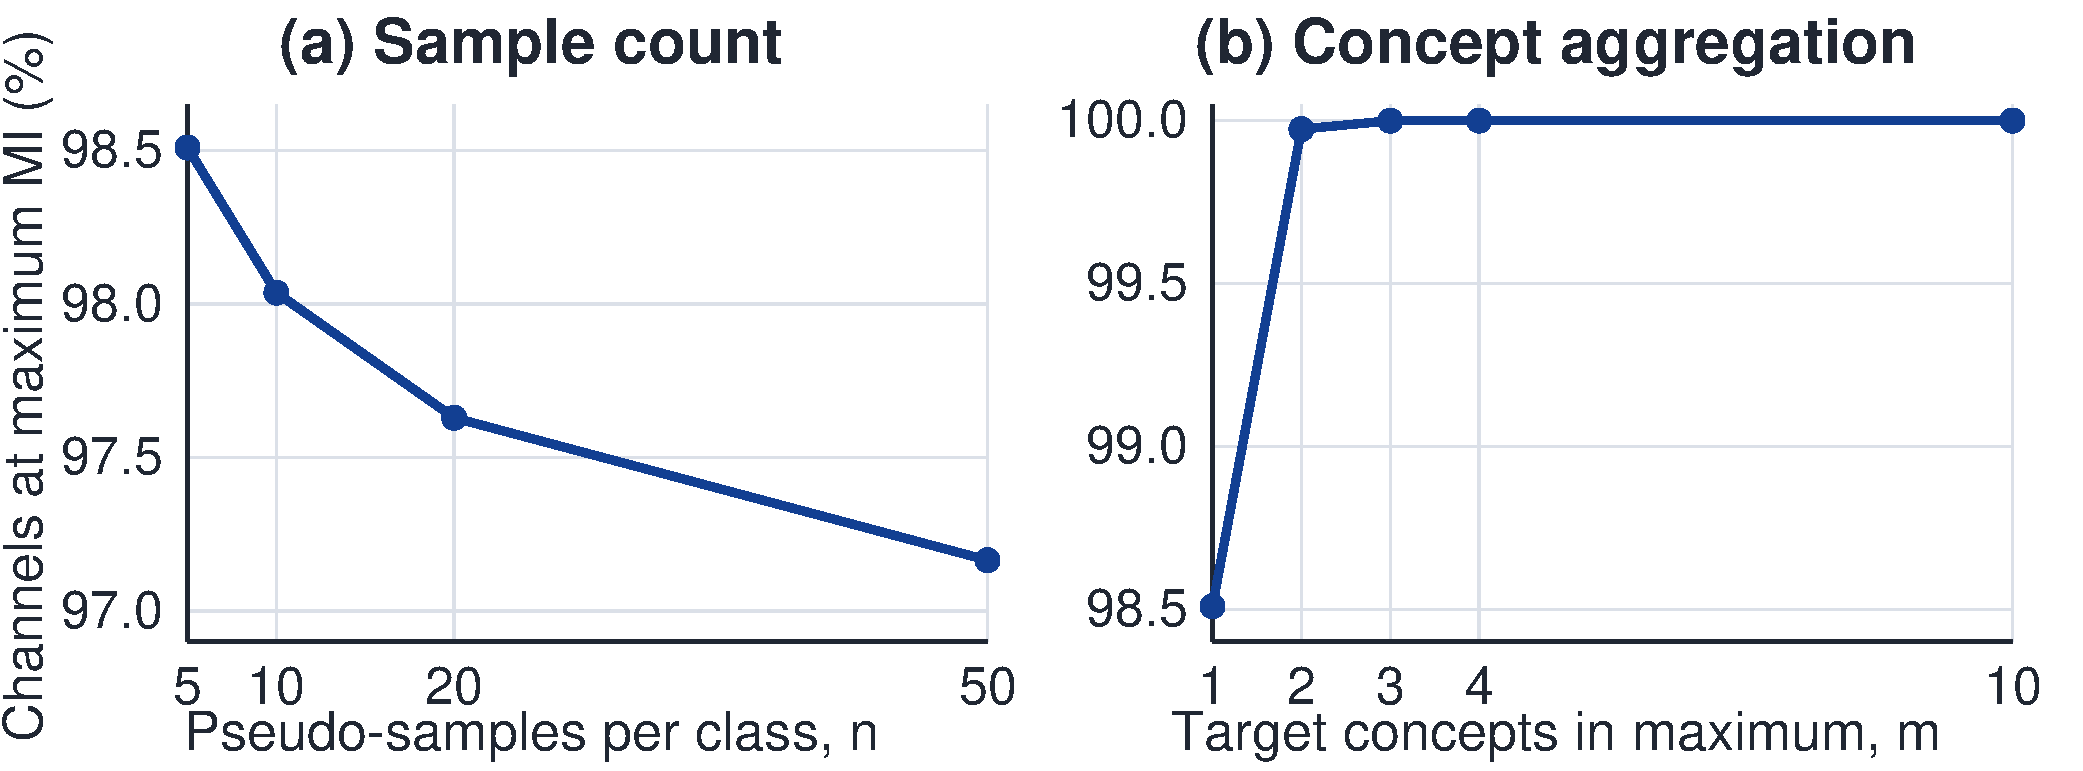
\includegraphics[width=0.97\linewidth]{figures/mi_saturation_panels.pdf}
\end{center}
\smalltext
Panel (a) increases the pseudo-sample count from $5+5$ to $50+50$, reducing the maximum-MI fraction only from $98.52\%$ to $97.17\%$. Panel (b) averages all target subsets of size $m$ across five seeds; every observed subset reaches $100\%$ saturation from $m=4$ onward.
\end{block}

\end{column}
\separatorcolumn

\begin{column}{\colwidth}
\setlength{\abovedisplayskip}{0.25em}
\setlength{\belowdisplayskip}{0.25em}
\setlength{\abovedisplayshortskip}{0.18em}
\setlength{\belowdisplayshortskip}{0.18em}

\begin{block}{5\quad Paper and Repository Weighting}
\blocktext
For $m$ target concepts, the paper defines the aggregate as
\[
MI_i^{(m)}=\max_{1\leq \ell\leq m}MI_i^{(\ell)}.
\]
In the measured ten-target data, every channel has reached $MI_i^{(m)}=\ln2$ by $m=4$. The paper's normalization therefore gives
\[
\alpha_i=\frac{\ln2}{\ln2}=1,
\qquad B=I,
\qquad
\operatorname{tr}(W^\top B W)=\lVert W\rVert_F^2.
\]
The repository instead applies, for each concept,
\[
MI\rightarrow z\text{-score}
\rightarrow \left[\operatorname{sigmoid}(\,\cdot\,/0.7)\right]^8
\rightarrow \max_\ell.
\]
The repository retains small channel-to-channel differences, so we next test whether their assignments matter.
\end{block}

\begin{block}{6\quad Final Channel Controls}
\blocktext
We evaluate Sections 6-7 on Stable Diffusion v1.5 with reconstructed ImageNet-Confuse5: 10 target concepts, 15 similar non-target concepts, and 120 images per concept and seed. Both tables report means over five fixed edit seeds.

The metrics are residual target accuracy $U\downarrow$, preserve accuracy $P\uparrow$, and
\[
O=\frac{2(100-U)P}{(100-U)+P}\uparrow.
\]
Constant mean and Identity $B$ change only the final $\alpha$.

\begin{center}
\tablefont
\renewcommand{\arraystretch}{1.20}
\begin{tabular}{p{0.43\linewidth}rrr}
\toprule
Variant & $U\downarrow$ & $P\uparrow$ & $O\uparrow$ \\
\midrule
Repository baseline & 19.27 & 40.46 & 53.90 \\
Constant mean & 19.18 & \textbf{40.81} & \textbf{54.23} \\
Identity $B$ (different scale) & 19.23 & 40.68 & 54.11 \\
\bottomrule
\end{tabular}
\end{center}

\smalltext
The controls that modify only the final weights remain near the baseline.
\end{block}

\begin{block}{7\quad Replacing Binary MI with Cosine Alignment}
\blocktext
Because binary MI saturates, we test a continuous channel score in the earlier per-concept mask; the final repository weights stay unchanged.

Let $w_i=W_{i:}$ and $d_\ell=c_\ell-c_0$, where $c_0$ is the empty-string vector. A continuous alignment score is
\[
r_i^{(\ell)}=
\frac{(w_i^\top d_\ell)^2}
{(\lVert w_i\rVert_2^2+\varepsilon)
 (\lVert d_\ell\rVert_2^2+\varepsilon)}
\approx\cos^2\theta_i.
\]
We test two replacements:
\[
\begin{aligned}
\text{Transformed cosine: }&\alpha^{(\ell)}=g(r^{(\ell)}),
&g(r)&=\left[\operatorname{sigmoid}\!\left(
\operatorname{z\text{-}score}(r)/0.7\right)\right]^8,\\
\text{Direct: }&\alpha^{(\ell)}=r^{(\ell)}.
\end{aligned}
\]
{\smalltext In $g$, z-scoring is across channels; the remaining operations are elementwise.\par}

\begin{center}
\tablefont
\renewcommand{\arraystretch}{1.16}
\begin{tabular}{p{0.43\linewidth}rrr}
\toprule
Variant & $U\downarrow$ & $P\uparrow$ & $O\uparrow$ \\
\midrule
Repository baseline & 19.27 & 40.46 & 53.90 \\
Transformed $\cos^2$ & 19.77 & \textbf{45.84} & \textbf{58.35} \\
Direct $\cos^2$ & \textbf{19.10} & 40.51 & 53.99 \\
\bottomrule
\end{tabular}
\end{center}

\smalltext
Transformed $\cos^2$ improves $P$ and $O$, but largely fails to erase tiger cat: $U$ rises by $40.17$ points on average. Direct $\cos^2$ avoids this failure but remains close to the baseline.
\end{block}

\begin{alertblock}{8\quad Conclusion}
\blocktext
\begin{itemize}
  \setlength{\itemsep}{0.20em}
  \item Binary MI barely distinguishes channels: saturation remains at $97.17\%$ with $50+50$ pseudo-samples, and the paper's aggregation gives $B=I$ from four targets onward.
  \item Changing only the final $\alpha$ has little effect; the repository's small channel differences show no clear image-level advantage.
  \item Cosine alignment changes the erase--preserve trade-off, but does not provide a reliable replacement.
\end{itemize}

\smalltext
Scope: SD v1.5, reconstructed Confuse5, and five fixed edit seeds.
\end{alertblock}

\begin{block}{Reference}
\blocktext
\smalltext
K. Deng et al., ``Forget Many, Forget Right: Scalable and Precise Concept Unlearning in Diffusion Models,'' \emph{ICLR}, 2026.
\end{block}

\end{column}
\separatorcolumn

\end{columns}
\end{frame}
\end{document}
